\documentclass{article}
\usepackage{ctex}
\usepackage{amsmath}
\usepackage{graphicx}
\usepackage{wrapfig}
\usepackage{caption}
\usepackage[top=0.8in, bottom=0.8in,left=0.8in, right=0.8in]{geometry}
\usepackage{float} 
% \usepackage{subwrapfigure}
\usepackage{subcaption}
\usepackage{bm}
\usepackage{geometry}
% \xeCJKsetup{CJKmath=true} 

\begin{document}
\section*{重力弹球(80分)}
弹球可以用来解决理论力学、拓扑、数论、几何问题。 假设碰撞是弹性的。  在这个系统中,粒子可以在边界上无限次弹跳。 在本题中,我们将考虑在存在重力场的情况下粒子在抛物面上的弹跳。这种系统出现在科学仪器的设计中,例如带有超冷中子的中子显微镜和用于捕获冷原子的存储腔。 在这两种情况下,粒子的能量都很低,以至于要考虑重力的作用。 \par
下假设旋转抛物面为
\[
M(x,y,z)=z-\dfrac{x^2+y^2}{4f}+f=0
\]
    \begin{center}
    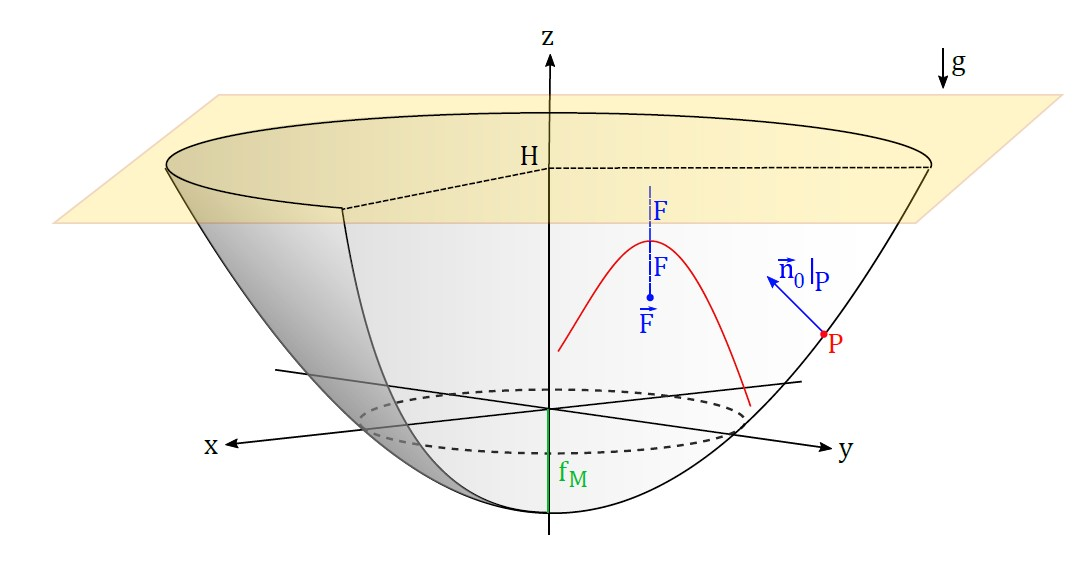
\includegraphics[scale=0.4]{img/1.jpg}\par
    \end{center}

\subsection*{PART.A\ \ 一些准备工作}
\begin{itemize}
    \item[(A.1)]对于旋转抛物面$M$上一点$P(x,y,z)$,请写出其单位法向量$\vec{n}|_P$.
    \item[(A.2)]请写出以速度$\vec{v}=(v_x,v_y,v_z)$起跳的质点的运动轨迹的半焦距$F$.\par (注:抛物线的标准方程为$x^2=2py$,其中$p$是焦距). 
    \item[(A.3)]设在$P(x,y,z)$发生碰撞。用碰撞前的速度$\vec{v}$与单位法向量$\vec{n}|_P$,写出碰撞后速度.
    \item[(A.4)]证明:碰撞前后$\hat{z}$方向角动量守恒. 
\end{itemize}
\subsection*{PART.B\ \ 一种特殊情况}
下面考虑碰撞点在一个固定的水平圆上的情况.为方便起见,现我们在极坐标系下考虑这个问题。如图将其投影在$xO'y$平面上。\par
    \begin{center}

\includegraphics[scale=0.3]{img/2.jpg}\par    
    \end{center}

\begin{itemize}
    \item[(B.1)]写出$\theta,v_r,v_{\phi}$之间的关系.
    \item[(B.2)]用$r_0,f_m,\theta$,写出$v_r,v_{\phi},v_z$.
    \item[(B.3)]写出轨迹的包络面(以$O'$为原点)  
    \begin{center}
    
\includegraphics[scale=0.4]{img/3.jpg}\par
    \end{center}

\end{itemize}
\subsection*{PART.C\ \ 二维抛物线内的弹球}
由于在三维中计算过于复杂,这里我们退而求其次,在二维中分析这个问题。\par
此时,抛物线方程可写作
\[
M(x,z)=z-\dfrac{x^2}{4f}+f=0
\]

\begin{itemize}
    \item[(C.1)]写出从同一点,以相同速度$v$抛出的粒子运动轨迹的焦点所构成的曲线.
    \item[(C.2)]考虑在$A$点发生的碰撞,$LA$为入射轨迹切线,$LM$为出射轨迹切线。$D$,$E$分别为入射出射轨迹的焦点,$BAC$为$M$在$A$处的切线,$KA$为竖直线.\par
    请证明:$\angle EAO=\angle OAD$(提示:利用抛物线的光学性质)
        \begin{center}
    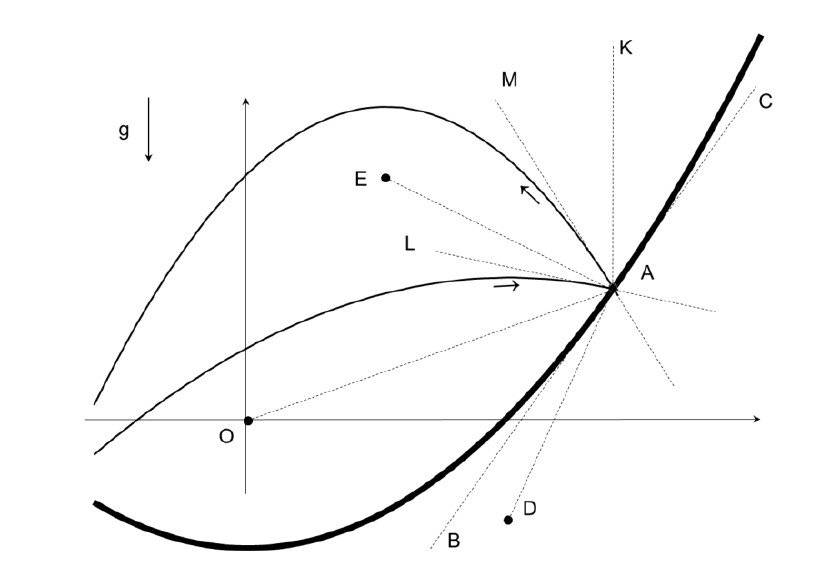
\includegraphics[scale=0.3]{img/4.jpg}\par    
    \end{center}

    \item[(C.3)]接上问,写出准线方程,并说出你的发现.
    \item[(C.4)]证明:运动轨迹的焦点到$O$的距离为定值
    \item[(C.5)]给定准线方程$y=H$,上问中的定值为$R$,写出包络线方程.(提示:有两条)
        \begin{center}
    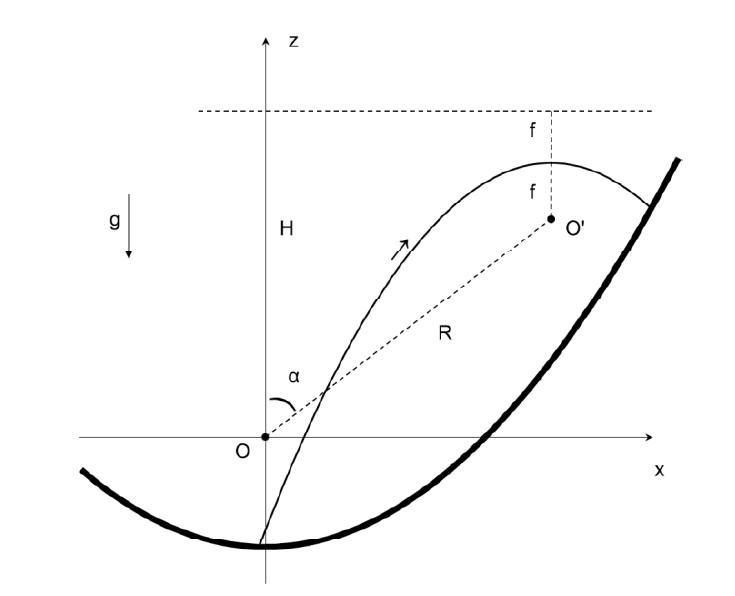
\includegraphics[scale=0.3]{img/5.jpg}\par    
    \end{center}

    \item[(C.6)]证明:相邻两次碰撞点在以$O$与轨迹焦点为焦点的椭圆上. 
    % \begin{wrapfigure}
        
    %     
\includegraphics[scale=0.25]{img/6.jpg}
    %     % \caption{}
    % \end{wrapfigure} 
        \begin{center}
    
\includegraphics[scale=0.3]{img/6.jpg}\par    
    \end{center}

\end{itemize}
\end{document} 